\documentclass{article}

\usepackage{tikz}
\usetikzlibrary{chains,
                positioning}

\begin{document}
    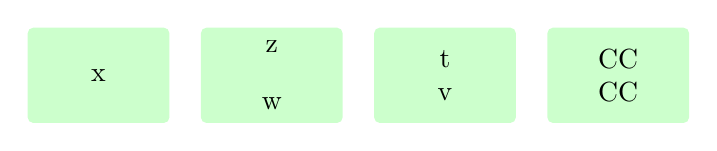
\begin{tikzpicture}[
node distance = 0mm and 4mm,
  start chain = going right,
    cc/.style = {fill=#1, rounded corners=2pt,
                 minimum height=1.21cm, minimum width=18mm, align=center,
                 inner sep=4, outer sep=0,
                 on chain},
    cc/.default = green!20
                        ]
\node[cc] (A) {x};
\node[cc] (B) {z\\[2ex] w}; % <---
\node[cc] (C) {t\\v};
\node[cc] (D) {CC\\ CC};
    \end{tikzpicture}
\end{document}